\section*{Standing questions}

\begin{frame}{Asymptotic behaviour?}
	\uncover<1->{
	    It is not yet safe to say that backreaction completely avoids instabilities of the solutions for each background electric field strength $\lambda$.
	}
	
	\uncover<2->{
	There are two main problems that can arise for a given configuration
	\begin{enumerate}
		\item The root finding algorithm for the boundary conditions finds no $\omega_1$
		\item There is no convergence
	\end{enumerate}
	

	These two issues can be solved by a smaller $\Delta \lambda$, or a relaxing parameter $c$ closer to 1.
}

	\uncover<2->{
		It can get however to the order of $\Delta \lambda \sim 10^{-7}$. 
}
\end{frame}

\begin{frame}{Good convergence}
\begin{figure}[h]
	\centering
	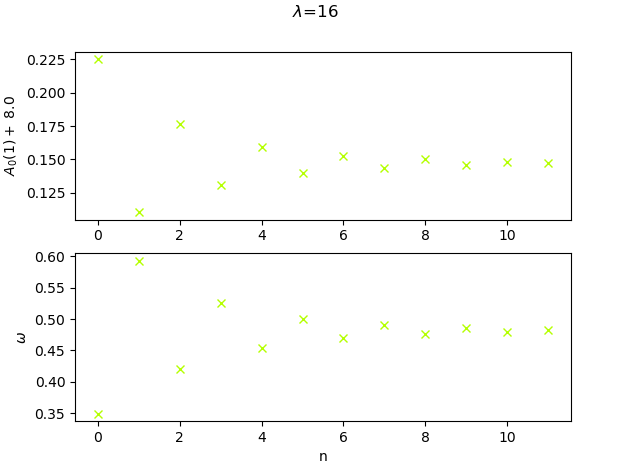
\includegraphics[width=0.5\textwidth]{figures/good-convergence.png}
	\caption{The iterations in the potential and the energy of the first mode in a case of good convergence.}
	\label{fig:figures-slow-convergence-png}
\end{figure}
\end{frame}

\begin{frame}{No convergence}
\begin{figure}[h]
	\centering
	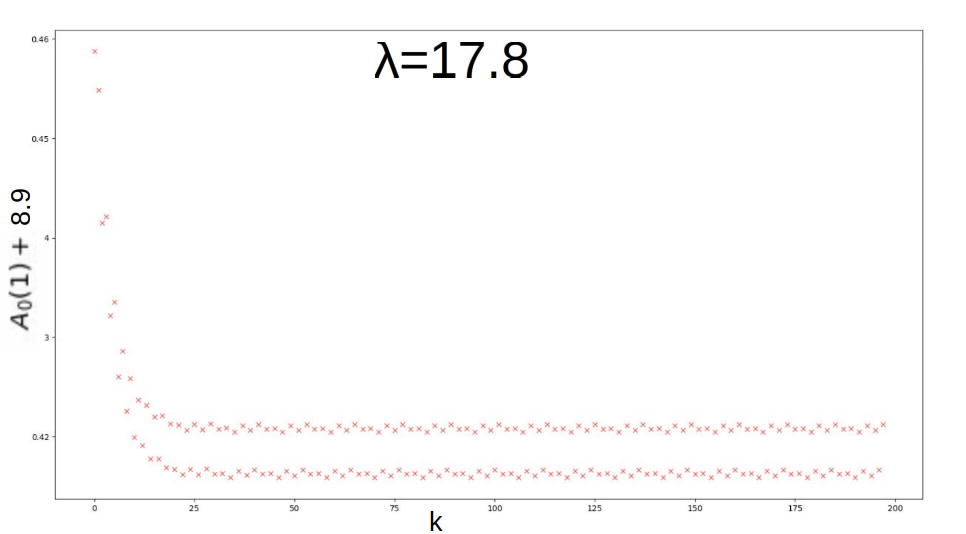
\includegraphics[width=0.6\textwidth]{figures/no-convergence.png}
	\caption{The values of the potential for constant $\lambda=17.8$, as $\kappa \to \infty$.}
	\label{fig:figures-slow-convergence-png}
\end{figure}
\end{frame}

\begin{frame}{Periodic points in the context of fixed points}

	\begin{columns}
	    \begin{column}{0.5\textwidth}
	    \begin{figure}[ht]
	        \centering
	        \incfig{the-periodic-points-of-the-functio1}
	        \caption{The periodic points of the function $f(x) = 1-x$}
	        \label{fig:the-periodic-points-of-the-functio}
	    \end{figure}
	    \end{column}
	    \begin{column}{0.5\textwidth}
	    Eventhough $x=\frac{1}{2}$ is a fixed point of $f(x)$, it cannot be found by taking the limit $\lim_{n \to \infty} f^n(x_1)$. Indeed, 
	    \begin{align*}
		    x_{2n}	&:= f^{2n}(x_1) = x_1 \\
		    x_{2n+1}	&:= f^{2n+1}(x_1) = 1- x_1 \\
	    \end{align*}
	    \end{column}
	\end{columns}
\end{frame}
\begin{frame}{Periodic points in the context of fixed points}

	\begin{columns}
	    \begin{column}{0.5\textwidth}
	    \begin{figure}[ht]
	        \centering
	        \incfig{the-periodic-points-of-the-functio2}
	        \caption{The periodic points of the function $f(x) = 1-x$}
	        \label{fig:the-periodic-points-of-the-functio}
	    \end{figure}
	    \end{column}
	    \begin{column}{0.5\textwidth}
	    Eventhough $x=\frac{1}{2}$ is a fixed point of $f(x)$, it cannot be found by taking the limit $\lim_{n \to \infty} f^n(x_1)$. Indeed, 
	    \begin{align*}
		    x_{2n}	&:= f^{2n}(x_1) = x_1 \\
		    x_{2n+1}	&:= f^{2n+1}(x_1) = 1- x_1 \\
	    \end{align*}
	    \end{column}
	\end{columns}
\end{frame}



\section*{Possible fixes}

\begin{frame}{Dynamic relaxation}
	In the 1-D case, no convergence appeared when $f'(x) = -1$.

	\uncover<2->{
	    Recall the relaxing update law 
	    \begin{align*}
	    	A_0^{\kappa+1} = c A_0^\kappa + (1-c)(A_\text{background}  + A^{\kappa}_\text{induced}), \hfill 0 < c \lesssim  1
	    \end{align*}
	}
	
	\uncover<3->{
	    Choose $c$ at every mesh point $z_n$, so that convergence is fastest, e.g. The convergence for the function $f(x) = \frac{1}{2}$ is immediate.
	}
\end{frame}

\begin{frame}{Extrapolation}
Since the problem arises from starting too far away from the next self consistent solution, try to predict by extrapolation.
\uncover<2->{
    \begin{themedTitleBlock}{Point-wise extrapolation}
    	$A_0^{\lambda_n}(z), A_0^{\lambda_{n-1}}(z)$ the self consistent potentials for $\lambda_n$, $\lambda_{n-1}$, respectively. Guess the next self consistent potential (and use it as a starting $A_0$ ) by 
    	\begin{align}
    		A_0^{\lambda_{n+1}}(z) = 
    		\frac{A_0^{\lambda_{n}}(z) -A_0^{\lambda_{n-1}}(z) }{\lambda_n - \lambda_{n-1}} (\lambda_{n+1}-\lambda_n) + A_0^{\lambda_n}(z) 
    	\end{align}
    \end{themedTitleBlock}
}

\end{frame}

\section{Upshot}

\begin{frame}
	\begin{itemize}
		\item We used the proper prescription for the vacuum polarization $ \left<\rho(z) \right>$ calculated in \cite{Wern2020}, to study the effect the backreaction of the Klein-Gordon field has on a background constant electric field. 
		\item We find that the backreaction raises the energy of the modes enough so as to avoid instabilities found when ignoring backreaction.
		\item However, convergence is still not fast enough to be able to correctly study the whole of the $\lambda$ parameter space.
	\end{itemize}
\end{frame}

\section{Outlook}

\begin{frame}
\begin{enumerate}
	\item Redoing the calculations for Neumann boundary conditions,
	\item Studying the effect of the size of the interval has for the different boundary conditions,
	\item Redoing the calculations for mixed (Robin) boundary conditions.
\end{enumerate}



\end{frame}
